\documentclass[]{article}
\usepackage[utf8]{inputenc}
\usepackage{polski}
\usepackage{listings}
\usepackage[usenames,dvipsnames]{xcolor}
\usepackage{geometry}
\usepackage{subcaption}
\usepackage{graphicx}
\usepackage{amsmath}
\usepackage{amssymb}
\usepackage{enumerate}
\DeclareGraphicsExtensions{.png}
\graphicspath{ {./} }
\geometry{
	a4paper,
	left=25mm,
	right = 25mm,
	top=25mm,
}
%%\hyphenchar\font=-1

\title{
	Sprawozdanie \\
	\large 
	Obliczenia naukowe - lista 3}
\author{Kamil Król}
\date{244949}


\begin{document}
	
	\maketitle
	
	\section*{Zadanie 1}
	Celem tego zadania było napisanie funkcji w języku Julia, która rozwiązuje równanie $f(x) = 0$ metodą bisekcji oraz opis tej metody.\\
	\textbf{Dane:}
	\begin{enumerate}[]
		\item $f(x)$ -- funkcja ciągła w przedziale $[a,b]$,
		\item $[a,b]$ -- przedział początkowy, w którym szukamy zera funkcji $f$ i który spełnia warunek $f(a)f(b)< 0$,
		\item $\epsilon, \delta$ -- dokładności obliczeń.
	\end{enumerate}
	\textbf{Opis:}\\
	Zanim przystąpimy do opisu tej metody przypomnijmy twierdzenie Darboux. Mówi ono, że jeżeli funkcja $f$ jest ciągła na przedziale $[a,b]$ i $f(a)f(b)<0$ czyli wartości funkcji $f$ na końcach przedziału mają różne znaki, to istnieje taki punkt $c\in[a,b]$, dla którego $f(c)=0$. Metoda bisekcji korzysta właśnie z tego twierdzenia do znalezienia miejsc zerowych funkcji $f$. Stąd biorą się wymagania co do danych tzn. funkcja $f$ ciagła na $[a,b]$ oraz warunek $f(a)f(b)< 0$. Metoda bisekcji polega na iteracyjnym połowieniu przedziału początkowego. Początkowy przedział $[a,b]$ spełnia warunek $f(a)f(b)< 0$ z warunków początkowych. Następnie ten przedział jest połowiony. W wyniku podziału otrzymujemy przedziały $[a,c]$ oraz $[c,b]$ gdzie $c$ jest środkiem przedziału $[a,b]$. Teraz musimy sprawdzić, który z tych przedziałów spełnia warunek mówiący o tym, że wartości funkcji $f$ na jego końcach mają różne znaki. Wybieramy przedział spełniający ten warunek i dla niego powtarzamy tę procedurę. Kończymy w momencie kiedy znajdziemy zero funkcji z zadaną dokładnością tj. $|f(c)|<\epsilon$ lub kiedy szerokość przedziału, w którym szukamy zera jest dostatecznie mała tzn. $b-a<\delta$.\\
	\textbf{Uwagi implementacyjne:}\\
	Na początek zastanówmy się w jaki sposób można obliczyć środek przedziału $[a,b]$. Najprostszą metodą wydaje się obliczenie średniej arytmetycznej tj. $c=\frac{a+b}{2}$. Z numerycznego punktu widzenia jest to metoda ryzykowna, gdyż w pewnych przypadkach moglibyśmy otrzymać środek przedziału $c$ nienależący do przedziału $[a,b]$. Dlatego środek przedziału obliczamy ze wzoru: $c = a + \frac{b-a}{2}$. Kolejnym niebezpieczeństwem jest sprawdzanie warunku $f(*)f(c)< 0$. Mnożenie po lewej stronie nierówności może w rezultacie dać nadmiar lub niedomiar. Można go uniknąć poprzez jawne sprawdzenie znaków $f(*)$ i $f(c)$ tj. $sign(f(*)) \neq sign(f(c))$.
	
	
	\clearpage
	
	\section*{Zadanie 2}
	
	Celem tego zadania było napisanie funkcji w języku Julia, która rozwiązuje równanie $f(x) = 0$ metodą Newtona oraz opis tej metody. Metoda Newtona nazywana jest też metodą stycznych.\\
	\textbf{Dane:}
	\begin{enumerate}[]
		\item $[a,b]$ -- przedział na którym wykonywać będziemy obliczenia,
		\item $f(x)$, $f'(x)$  -- funkcja $f$ należąca do klasy $C^2[a,b]$ oraz pochodna funkcji $f$
		\item $x_0$ -- przybliżenie początkowe,
		\item $\epsilon, \delta$ -- dokładności obliczeń,
		\item \texttt{maxit} -- maksymalna dopuszczalna liczba iteracji.
	\end{enumerate}
	\textbf{Opis:}\\
	Dodatkowym założeniem jest to, że szukamy pierwiastka $r$ dla którego $f'(r)\ne0$, tzn. pierwiastek $r$ jest pierwiastkiem jednokrotnym. Metoda Newtona opiera się na linearyzacji funkcji (zastąpieniu jej funkcją liniową) przez użycie jej rozwinięcia w szereg Taylora.
	$$f(x) = f(x_n ) + f'(x_n )(x-x_n) + O((x-x_n )^2)\text{ -- rozwinięcie w szereg Taylora}$$
	$$f(x)\approx f(x_n ) + f'(x_n )(x-x_n) \text{ -- linearyzacja}$$
	Mamy zatem równianie $f(x_n ) + f'(x_n )(x_{n+1}-x_n) = 0$ co po przekształceniu daje wzór rekurencyjny $x_{n+1} = x_n - \dfrac{f(x_n)}{f'(x_n)}$. Jest to wzór na kolejne przybliżenia zera funkcji. Widać, też dlaczego pojawia się założenie o tym że $f'(r)\ne0$ -- dzielilibyśmy wtedy przez 0. Zauważmy teraz, że styczna do wykresu funkcji $f$ w punkcie $x_n$ przecina oś OX w punkcie $(x_{n+1},0)$. Stąd właśnie bierze się alternatywna nazwa metody Newtona - metoda stycznych.
	\begin{figure}[!htbp]
		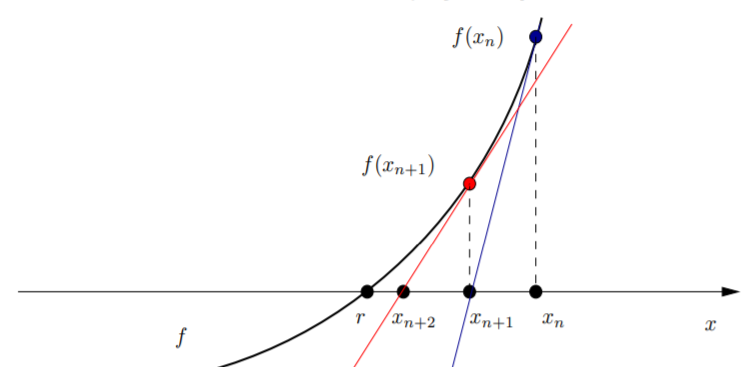
\includegraphics[scale=0.7]{newton}
		\centering
		\caption{Interpretacja graficzna metody Newtona -- grafika z wykładu}
	\end{figure}
	Na początku algorytmu następuje sprawdzenie czy wartość $f(x_0)$ jest dostatecznie bliska zeru tzn. $|f(x_0)|<\epsilon$. Jeśli tak to kończymy pracę algorytmu i zwracamy wynik. W przeciwnym wypadku przystępujemy do następnego kroku i sprawdzamy czy wartość pochodnej nie jest zbyt bliska zeru tj. $|f'(x_0)|<\epsilon$. Jeśli by się tak stało dalsze obliczenia nie miałyby sensu. Następnie używając podanego wcześniej wzoru rekurencyjnego wyliczamy iteracyjnie kolejne przybliżenia pierwiastka. Robimy to dopóki nie osiągniemy pożądanej dokładności tj. $|f(x_n)|<\epsilon$ lub nie otrzymamy dostatecznie bliskich sobie przybliżeń tj. $|x_n-x_{n-1}|<\delta$. Jeśli nie uda się spełnić tych warunków w dopuszczalnej liczbie iteracji przerywamy obliczenia. Szczególną sytuacją kiedy nie uda nam się spełnić tych warunków jest to kiedy metoda Newtona okazuje się rozbieżna dla zadanego $x_0$. Inaczej mówiąc, może się tak zdażyć, że dla zadanego przybliżenia początkowego $x_0$ metoda Newtona nie jest zbieżna. Widać zatem, że nie jest to metoda zbieżna globalnie. Dlatego właśnie stosuje się ją często w połączeniu z inna metodą zbieżną globalnie.
	Metoda Newtona jest szybsza niż metoda bisekcji, ponieważ ma kwadratowy współczynnik zbieżności.
	\\
	%\textbf{Uwagi implementacyjne:}\\

	\section*{Zadanie 3} 
	
	Celem tego zadania było napisanie funkcji w języku Julia, która rozwiązuje równanie $f(x) = 0$ metodą siecznych oraz opis tej metody.\\
	\textbf{Dane:}
	\begin{enumerate}[]
		\item $[a,b]$ -- przedział na którym wykonywać będziemy obliczenia,
		\item $f(x)$ -- funkcja $f$ należąca do klasy $C^2[a,b]$,
		\item $x_0$, $x_1$ -- przybliżenia początkowe,
		\item $\epsilon, \delta$ -- dokładności obliczeń,
		\item \texttt{maxit} -- maksymalna dopuszczalna liczba iteracji.
	\end{enumerate}
	\textbf{Opis:}\\
	Dodatkowym założeniem jest to, że szukamy pierwiastka $r$ dla którego $f'(r)\ne0$, tzn. pierwiastek $r$ jest pierwiastkiem jednokrotnym -- tak samo jak dla metody Newtona.
	Zanim przystąpimy do opisu metody siecznych przyjrzyjmy się jeszcze raz metodzie Newtona. Wadą metody Newtona jest konieczność obliczenia pochodnej funkcji $f$. Metoda siecznych różni się od metody Newtona tym, że zamiast obliczać wartość $f'(x_n)$, aproksymujemy ją używając następującej formuły: $f'(x_n) \approx \dfrac{f(x_n)-f(x_{n-1})}{x_n-x_{n-1}}$. Przypomnijmy, że w metodzie Newtona kolejne przybliżenia otrzymywaliśmy ze wzoru rekurencyjnego: $x_{n+1} = x_n - \dfrac{f(x_n)}{f'(x_n)}$. Kiedy pochodną funkcji $f$ zastąpimy powyższym przybliżeniem otrzymujemy wzór: $x_{n+1} := x_n - f(x_n)\dfrac{x_n-x_{n-1}}{f(x_n)-f(x_{n-1})}$. Widzimy zatem, że metoda siecznych jest modyfikacją meotdy Newtona, która \textit{ucieka} od liczenia wartości pochodnej funkcji $f$. Kiedy przyjrzymy się dokładniej otrzymanemu wzorowi rekurencyjnemu widzimy, że pojawiła się potrzeba znajomości dwóch poprzednich wartości $x$. Dlatego właśnie w danych pojawia się $x_0$, $x_1$. Warunkiem końcowym jest znalezienie pierwiastka z pożądaną dokładnością tj. $|f(x_n)|<\epsilon$ lub otrzymanie dostatecznie bliskich sobie przybliżeń tj. $|x_n-x_{n-1}|<\delta$. (Warunki takie same jak dla metody Newtona). Może się zdarzyć, że dla zadanych przybliżeń początkowych metoda siecznych nie jest zbieżna, ponieważ metoda siecznych nie jest zbieżna globalnie. Zatem w przypadku nieosiągnięcia warunków końcowych w maksymalnej dopuszczalnej liczbie iteracji zwracany jest błąd. Współczynnik zbieżności metody siecznych wynosi $\alpha = \frac{1+\sqrt{5}}{2}\approx1.618$. 
	Interpretacja graficzna tej metody wygląda w następujący sposób. Każne kolejne przybliżenie pierwiastka $x_{n+2}$ to przecięcie siecznej poprowadzonej przez punkty $(x_n$, $f(x_n))$ i $(x_{n+1}$, $f(x_{n+1}))$, gdzie $x_n$ i $x_{n+1}$ to dwa poprzednie przybliżenia, z osią OX. Poniżej grafika.
	\begin{figure}[!htbp]
		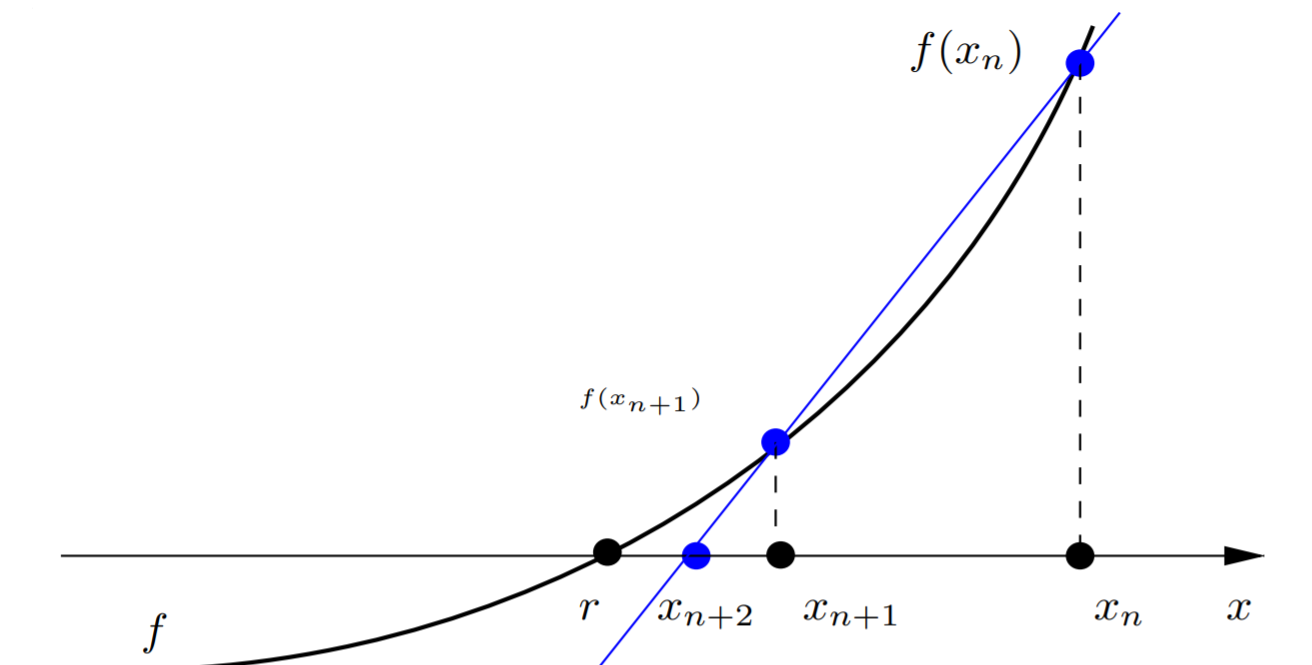
\includegraphics[scale=0.59]{secant}
		\centering
		\caption{Interpretacja graficzna metody siecznych -- grafika z wykładu}
	\end{figure}
	\clearpage

	\noindent\textbf{Uwagi implementacyjne:}\\
	W implementacji tej metody dodano warunek mówiący, że kolejne wartości bezwzględne wartości funkcji tworzą ciąg nierosnący tzn. $|f(x_n)| \leq |f(x_{n+1})|$. W przypadku kiedy trafią się wartości $x_n$ i $x_{n+1}$, które nie spełniają tego warunku, są one ze sobą zamieniane.
	
	
	
	
	\section*{Zadanie 4}

	Celem zadania było wyznaczenie pierwiastków równania $\sin{x}-(\frac{1}{2}x)^2 = 0$ używając wcześniej zaimplementowanych metod:
	\begin{enumerate}[(a)]
		\item metody bisekcji (z przedziałem początkowym $[1.5, 2.0]$),
		\item metody Newtona (z przybliżeniem początkowym $x_0 = 1.5$),  
		\item metody siecznych (z przybliżeniami początkowymi $x_0 = 1.0$ i $x_1 = 2.0$).
	\end{enumerate}
	Dla wszystkich metod dokładności były wspólne tj. $\delta = \epsilon = \frac{1}{2}10^{-5}$. Za maksymalną liczbę iteracji przyjąłem 40. Zacząłem od obliczenia pochodnej funkcji $f$, $f'(x) = \cos{x} - \frac{1}{2}x$ potrzebnej w metodzie Newtona. Wyniki działania programów znajdują się w tabeli poniżej.
	
	\begin{table}[h!]
		\centering
		\label{tab:table1}
		\begin{tabular}{|c|c|c|c|}
			\hline
			metoda & wartość pierwiastka - $r$ & wartość funkcji w punkcie $r$ - $f(r)$ & liczba iteracji \\ \hline
			metoda bisekcji & 1.9337539672851562 & -2.7027680138402843e-7 & 16 \\ \hline
			metoda Newtona & 1.933753779789742 & -2.2423316314856834e-8 & 4 \\ \hline
			metoda siecznych & 1.933753644474301 & 1.564525129449379e-7 & 4 \\ \hline
		\end{tabular}
	\end{table}
	
	Widać, że różnica w ilości wykonanych iteracji między metodą bisekcji a dwoma pozostałymi jest znaczna. Metoda bisekcji okazała się najwolniejsza. Metody Newtona i siecznych okazały się w tym przypadku porównywalne jeśli chodzi o ilość iteracji potrzebną do osiągnięcia zadanej dokładności. Wyniki eksperymentu mają odzwierciedlenie w teorii. Współczynnik zbieżności dla metody siecznych wynosi $1$ (zbieżność liniowa), dla metody Newtona $2$ (zbieżność kwadratowa), a dla metody siecznych $\approx1.62$.
	
	\clearpage
	
	\section*{Zadanie 5}
	Celem zadania było użycie metody bisekcji do znalezienia, wartości zmiennej $x$, dla której przecinają się wykresy funkcji $y=3x$ oraz $y=e^x$. Zadane dokładności wynosiły $\delta = \epsilon = 10^{-4}$. Zadanie można sprowadzić do problemu rozwiązania równania $e^x - 3x = 0$ lub równoważnie znalezienia miejsc zerowych funkcji $f(x) = e^x - 3x$. Pierwszą rzeczą jaką należało wykonać to dobrać przedział lub przedziały początkowe. Wiemy, że metoda bisekcji wymaga takiego przedziału, że wartości funkcji w jego końcach mają różny znak. W celu wyznaczenia przedziałów początkowych posłużyłem się poniższymi wykresami.
	
	\begin{figure}[!htbp]
		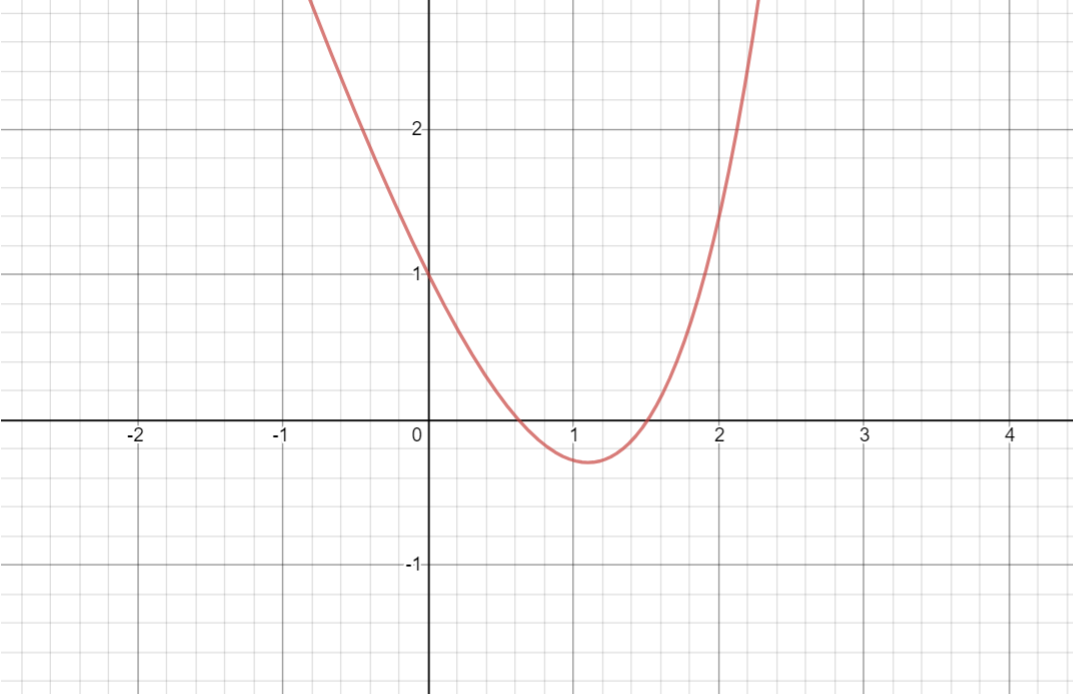
\includegraphics[width=\textwidth]{task5plot}
		\centering
		\caption{Wykres funkcji $f(x) = e^x - 3x$}
	\end{figure}
	
%	\begin{figure}[!htbp]
%		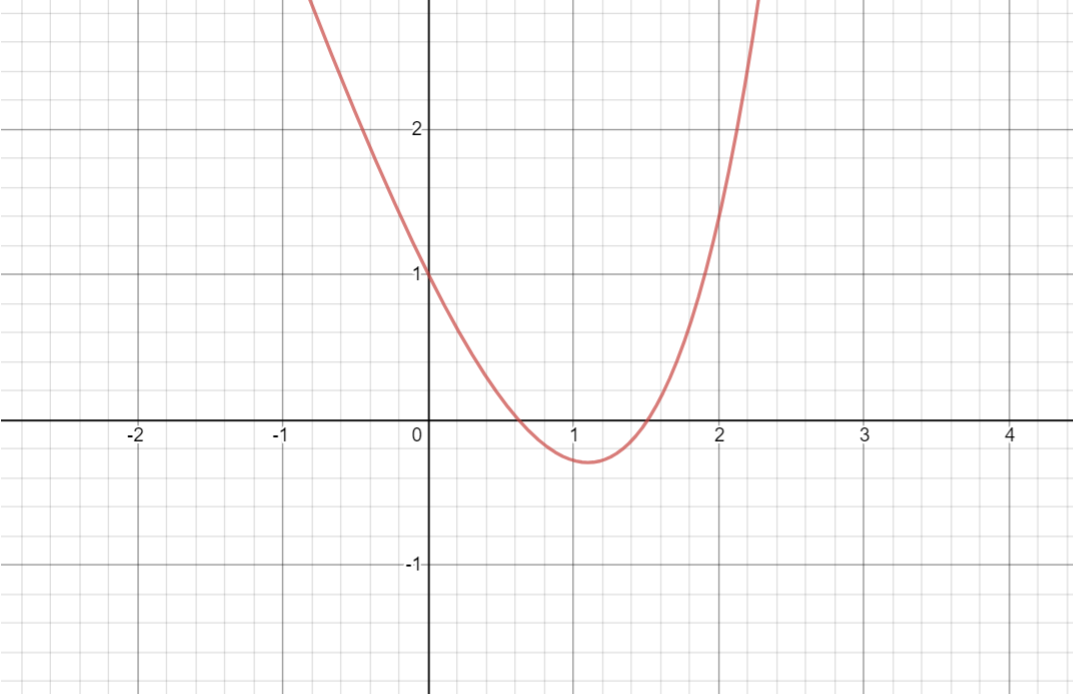
\includegraphics[height=0.38\textheight]{task5plot}
%		\centering
%		\caption{Wykres funkcji $f(x) = e^x - 3x$}
%	\end{figure}
%	\begin{figure}[!htbp]
%		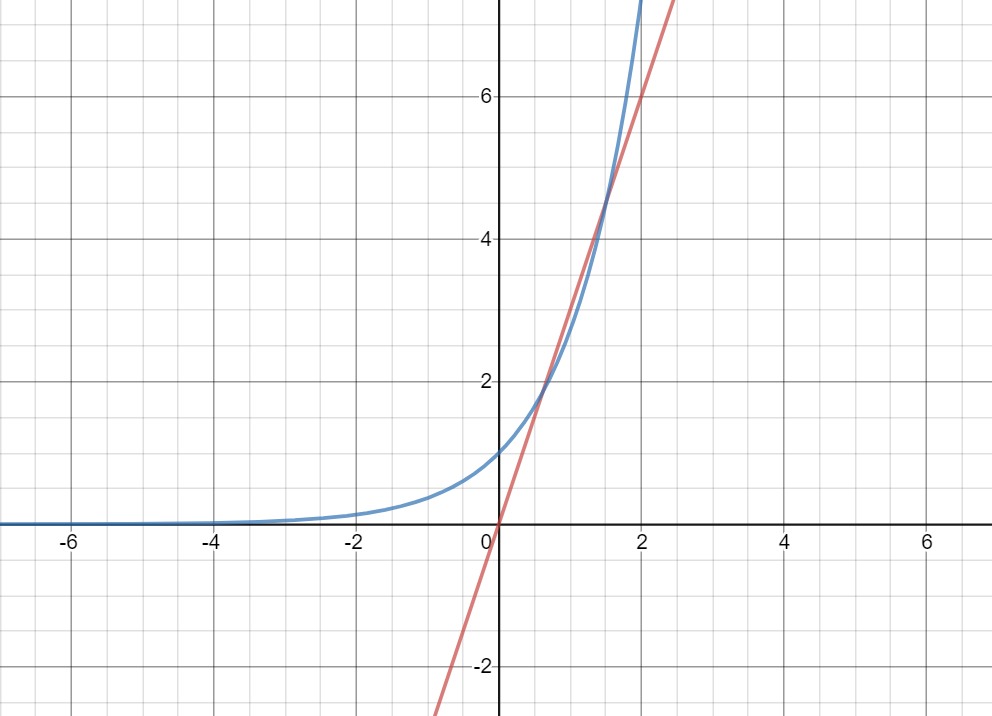
\includegraphics[height=0.36\textheight]{3xexplot}
%		\centering
%		\caption{Wykresy funkcji $e^x$ i $3x$}
%	\end{figure}

	Patrząc na wykresy wybrałem przedziały [0,1] oraz [1,2]. Oba z nich spełniają wymagania metody bisekcji. Znalezione pierwiastki to $x_1=0.619140625$ oraz $x_2=1.5120849609375$ co pokrywa się z tym co sugeruje wykres.
	
	
	\begin{table}[!h]
		\centering
		\label{tab:table1}
		\begin{tabular}{c|c|c}
			
			 & $x_1$ & $x_2$ \\ \hline
			Wartość pierwiastka $r$ &  0.619140625 & 1.5120849609375 \\ 
			Wartość funkcji $f(r)$ & -9.066320343276146e-5 & -7.618578602741621e-5  \\ 
			Liczba iteracji & 9 & 13 \\
			Przedział & [0,1] & [1,2] \\
		\end{tabular}
	\end{table}

	Widać, że oba pierwiastki występują dość blisko siebie oraz fakt, że znacznym ułatwieniem w znaleznieniu przedziałów początkowych była znajomość przebiegu funkcji $f$. Na wykresie od razu widać było, że powinniśmy się spodziewać dokładnie dwóch miejsc zerowych oraz gdzie się ich spodziewać. Bez pomocy jaką była znajomość przebiegu funkcji $f$ nie wiedzielibyśmy nawet ilu miejsc zerowych powinniśmy się spodziewać. Innym wnioskiem jest fakt, że znalezione miejsce zerowe zależy od wybranego przedziału początkowego. Ogólniejszym wnioskiem jest to, że bez dobrej znajomości przebiegu funkcji metoda bisekcji może być problematyczna do zastosowania. 

	\clearpage
	
	\section*{Zadanie 6}
	
	Celem zadania było sprawdzenie zachowania pewnego równania rekurencyjnego poprzez wykonanie 40 iteracji dla podanych w treści zadania zestawów danych. Równanie:
	$$x_{n+1} := x^2_n + c, \ \textrm{dla} \ n = 0,1,\dots$$
	
	Wyniki znajdują się w tabelach na końcu paragrafu.
	
	

	Obserwując wyniki dla c = -2 widać, że dla $x_0 = 1$ oraz dla $x_0 = 2$ rekurencja okazała się stabilna. Inna rzecz jaką można zauważyć, to fakt, że dla wartości nieznacznie odchylonej od 2.0 tzn. $x_0 = 1.99999999999999$ wyniki są zupełnie różne niż dla $x_0 = 2$. Widać zatem bardzo dużą czułość na warunki początkowe. Obserwując wyniki dla $c = -1$ widać, że otrzymane ciągi dla $x_0 = 1$ jak i $x_0 = -1$ są identyczne. Wynika to z podnoszenia tej wartości do kwadratu. Ostatnie dwie kolumny pokazują sytuację gdzie oba ciągi po jakimś czasie się stabilizują. Zarówno dla $x_0 = 0.25$ jak i $x_0 = 0.75$ otrzymujemy naprzemienne ciągi -1 i 1. Poniżej iteracje graficzne.
	

\begin{figure}[!htbp]
	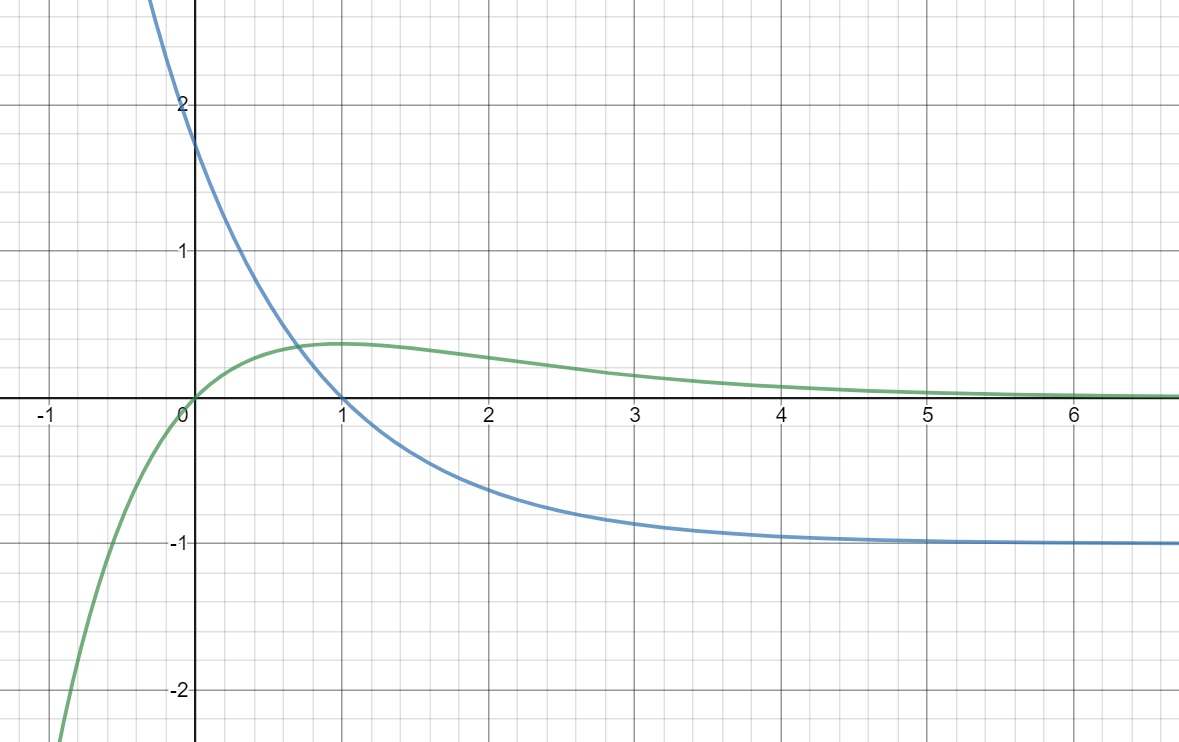
\includegraphics[scale=1]{e1-x-1andxe-x.png}
	\centering
	\caption{$c = -2$, $x_0 = 1$}
\end{figure}

Wnioski. Zauważmy, że w tym zadaniu również mamy do czynienia ze zjawiskiem sprzężenia zwrotnego. W całym zadaniu możemy wyróżnić 3 typy doświadczeń. Pierwszy z nich to dwa pierwsze doświadczenia oraz te z c = -1 i $x_0 \in \{-1,1\}$, w którch otrzymano ciągi stałe lub naprzemienne, są to układy stabilne. Zauważmy też, że punkty $-1$ i $2$ są punktami stałymi funkcji $x^2 - 2$. Właśnie dlatego w dwóch pierwszych doświadczeniach wartości zbiegają do tych wartości. Drugi typ to doświadczenie z $x_0 = 1.99999999999999$. Tutaj ciąg był chaotyczny. Jest to układ niestabilny. Trzeci typ doświadczenia reprezentują dwa ostatnie eksperymenty. W obu z nich układ początkowo był chaotyczny, ale po którymś kroku zaczął się stabilizować. Są to układy stabilne.

	
	\begin{table}[!h]
		\centering
		\label{tab:table1}
		\begin{tabular}{|c|c|c|c|}
			\multicolumn{4}{c}{$c = -2$} \\
			\hline
			numer iteracji & $x_0 = 1$ & $x_0 = 2$ & $x_0 = 1.99999999999999$\\
			\hline
			1 & -1 &	 2 &	 1.99999999999996 \\ \hline
			2 & -1 &	 2 &	 1.9999999999998401 \\ \hline
			3 & -1 &	 2 &	 1.9999999999993605 \\ \hline
			4 & -1 &	 2 &	 1.999999999997442 \\ \hline
			5 & -1 &	 2 &	 1.9999999999897682 \\ \hline
			6 & -1 &	 2 &	 1.9999999999590727 \\ \hline
			7 & -1 &	 2 &	 1.999999999836291 \\ \hline
			8 & -1 &	 2 &	 1.9999999993451638 \\ \hline
			9 & -1 &	 2 &	 1.9999999973806553 \\ \hline
			10 & -1 &	 2 &	 1.999999989522621 \\ \hline
			11 & -1 &	 2 &	 1.9999999580904841 \\ \hline
			12 & -1 &	 2 &	 1.9999998323619383 \\ \hline
			13 & -1 &	 2 &	 1.9999993294477814 \\ \hline
			14 & -1 &	 2 &	 1.9999973177915749 \\ \hline
			15 & -1 &	 2 &	 1.9999892711734937 \\ \hline
			16 & -1 &	 2 &	 1.9999570848090826 \\ \hline
			17 & -1 &	 2 &	 1.999828341078044 \\ \hline
			18 & -1 &	 2 &	 1.9993133937789613 \\ \hline
			19 & -1 &	 2 &	 1.9972540465439481 \\ \hline
			20 & -1 &	 2 &	 1.9890237264361752 \\ \hline
			21 & -1 &	 2 &	 1.9562153843260486 \\ \hline
			22 & -1 &	 2 &	 1.82677862987391 \\ \hline
			23 & -1 &	 2 &	 1.3371201625639997 \\ \hline
			24 & -1 &	 2 &	 -0.21210967086482313 \\ \hline
			25 & -1 &	 2 &	 -1.9550094875256163 \\ \hline
			26 & -1 &	 2 &	 1.822062096315173 \\ \hline
			27 & -1 &	 2 &	 1.319910282828443 \\ \hline
			28 & -1 &	 2 &	 -0.2578368452837396 \\ \hline
			29 & -1 &	 2 &	 -1.9335201612141288 \\ \hline
			30 & -1 &	 2 &	 1.7385002138215109 \\ \hline
			31 & -1 &	 2 &	 1.0223829934574389 \\ \hline
			32 & -1 &	 2 &	 -0.9547330146890065 \\ \hline
			33 & -1 &	 2 &	 -1.0884848706628412 \\ \hline
			34 & -1 &	 2 &	 -0.8152006863380978 \\ \hline
			35 & -1 &	 2 &	 -1.3354478409938944 \\ \hline
			36 & -1 &	 2 &	 -0.21657906398474625 \\ \hline
			37 & -1 &	 2 &	 -1.953093509043491 \\ \hline
			38 & -1 &	 2 &	 1.8145742550678174 \\ \hline
			39 & -1 &	 2 &	 1.2926797271549244 \\ \hline
			40 & -1 &	 2 &	 -0.3289791230026702 \\ \hline
		\end{tabular}
	\end{table}


\end{document}